%!TEX TS-program = xelatex
\documentclass[12pt, a4paper, oneside]{article}

\usepackage{amsmath,amsfonts,amssymb,amsthm,mathtools}  % пакеты для математики

\usepackage[english, russian]{babel} % выбор языка для документа
\usepackage[utf8]{inputenc} % задание utf8 кодировки исходного tex файла
\usepackage[X2,T2A]{fontenc}        % кодировка

\usepackage{fontspec}         % пакет для подгрузки шрифтов
\setmainfont{Linux Libertine O}   % задаёт основной шрифт документа

\usepackage{unicode-math}     % пакет для установки математического шрифта
\setmathfont[math-style=upright]{Neo Euler} % шрифт для математики

% Конкретный символ из конкретного шрифта
% \setmathfont[range=\int]{Neo Euler}

%%%%%%%%%% Работа с картинками %%%%%%%%%
\usepackage{graphicx}                  % Для вставки рисунков
\usepackage{graphics}
\graphicspath{{images/}{pictures/}}    % можно указать папки с картинками
\usepackage{wrapfig}                   % Обтекание рисунков и таблиц текстом

%%%%%%%%%%%%%%%%%%%%%%%% Графики и рисование %%%%%%%%%%%%%%%%%%%%%%%%%%%%%%%%%
\usepackage{tikz, pgfplots}  % язык для рисования графики из latex'a

%%%%%%%%%% Гиперссылки %%%%%%%%%%
\usepackage{xcolor}              % разные цвета

\usepackage{hyperref}
\hypersetup{
	unicode=true,           % позволяет использовать юникодные символы
	colorlinks=true,       	% true - цветные ссылки, false - ссылки в рамках
	urlcolor=blue,          % цвет ссылки на url
	linkcolor=red,          % внутренние ссылки
	citecolor=green,        % на библиографию
	pdfnewwindow=true,      % при щелчке в pdf на ссылку откроется новый pdf
	breaklinks              % если ссылка не умещается в одну строку, разбивать ли ее на две части?
}


\usepackage{todonotes} % для вставки в документ заметок о том, что осталось сделать
% \todo{Здесь надо коэффициенты исправить}
% \missingfigure{Здесь будет Последний день Помпеи}
% \listoftodos --- печатает все поставленные \todo'шки

\usepackage[paper=a4paper, top=20mm, bottom=15mm,left=20mm,right=15mm]{geometry}
\usepackage{indentfirst}       % установка отступа в первом абзаце главы

\usepackage{setspace}
\setstretch{1.15}  % Межстрочный интервал
\setlength{\parskip}{4mm}   % Расстояние между абзацами
% Разные длины в латехе https://en.wikibooks.org/wiki/LaTeX/Lengths


\usepackage{xcolor} % Enabling mixing colors and color's call by 'svgnames'

\definecolor{MyColor1}{rgb}{0.2,0.4,0.6} %mix personal color
\newcommand{\textb}{\color{Black} \usefont{OT1}{lmss}{m}{n}}
\newcommand{\blue}{\color{MyColor1} \usefont{OT1}{lmss}{m}{n}}
\newcommand{\blueb}{\color{MyColor1} \usefont{OT1}{lmss}{b}{n}}
\newcommand{\red}{\color{LightCoral} \usefont{OT1}{lmss}{m}{n}}
\newcommand{\green}{\color{Turquoise} \usefont{OT1}{lmss}{m}{n}}

\usepackage{titlesec}
\usepackage{sectsty}
%%%%%%%%%%%%%%%%%%%%%%%%
%set section/subsections HEADINGS font and color
\sectionfont{\color{MyColor1}}  % sets colour of sections
\subsectionfont{\color{MyColor1}}  % sets colour of sections

%set section enumerator to arabic number (see footnotes markings alternatives)
\renewcommand\thesection{\arabic{section}.} %define sections numbering
\renewcommand\thesubsection{\thesection\arabic{subsection}} %subsec.num.

%define new section style
\newcommand{\mysection}{
	\titleformat{\section} [runin] {\usefont{OT1}{lmss}{b}{n}\color{MyColor1}} 
	{\thesection} {3pt} {} } 


%	CAPTIONS
\usepackage{caption}
\usepackage{subcaption}
%%%%%%%%%%%%%%%%%%%%%%%%
\captionsetup[figure]{labelfont={color=Turquoise}}

\pagestyle{empty}

%%%%%%%%%% Свои команды %%%%%%%%%%
\usepackage{etoolbox}    % логические операторы для своих макросов

% Все свои команды лучше всего определять не по ходу текста, как это сделано в этом документе, а в преамбуле!

% Одно из применений - уничтожение какого-то куска текста!
\newbool{answers}
\booltrue{answers}
%\boolfalse{answers}

% бульпоинты в списках
\definecolor{myblue}{rgb}{0, 0.45, 0.70}
\newcommand*{\MyPoint}{\tikz \draw [baseline, fill=myblue,draw=blue] circle (2.5pt);}
\renewcommand{\labelitemi}{\MyPoint}

\begin{document}
	
\section*{Семинар 4-5: Продажи и линейная регрессия }

\subsection*{Задача 1}

Предположим, Олег хочет купить автомобиль и считает сколько денег ему нужно для этого накопить\footnote{сделано по мотивам \url{https://vas3k.ru/blog/machine_learning/}}. Он пересмотрел десяток объявлений в интернете и увидел, что новые автомобили стоят около $20 000$, годовалые — примерно $19 000$, двухлетние — $18 000$ и так далее.

В уме Олег-аналитик выводит формулу: адекватная цена автомобиля начинается от $20 000$ и падает на $1000$ каждый год, пока не упрётся в $10 000$. Олег сделал то, что в машинном обучении называют регрессией — предсказал цену по известным данным. Давайте попробуем повторить подвиг Олега.

\begin{enumerate}
	\item[а)] Как выглядит формула в случае Олега?
	\item[б)] За сколько продать старый афон? Как выглядит формула?
	\item[в)] Сколько шашлыка брать на дачу? Как выглядит формула?
	\item[г)] Сколько брать шашлыка, если есть толстый друг? Как можно назвать толстого друга в терминах машинного обучения? Испортит ли толстый друг формулу?
	\item[д)] Сколько одежды брать с собой в путешествие? 
\end{enumerate}

Было бы удобно иметь формулу под каждую проблему на свете. Но взять те же цены на автомобили: кроме пробега есть десятки комплектаций, разное техническое состояние, сезонность спроса и еще столько неочевидных факторов, которые Олег, даже при всём желании, не учел бы в голове. Люди тупы и ленивы — надо заставить вкалывать роботов.

\ifbool{answers}{
	\textbf{Решение:}

\begin{enumerate}
	\item[а)]  Формула Олега: $y_i = 20000 - 1000 \cdot x_i$, где $y_i$--- цена машины, $x_i$ --- её возраст. Если бы мы собрали данные о машинах и загнали их в компьютер, нам нужно было бы оценить модель
	
	\[ y_i = \beta_0 + \beta_1 \cdot  x_i.\]
	
	Коэффициент $\beta_0$ отражает базовую стоимость машины, а $\beta_1$ то, насколько она дешевеет с каждым годом. 
		
	\item[б)]  Я не знаю, к чему мы пришли при обсуждении на семинаре, но скорее всего к чему-то похожему на случай Олега. 
	
	\item[в)]   Это зависит от числа людей и числа дней, на которое мы едем на дачу. Наверное логично было бы брать полкило на человека в день, то есть $y_i = 0.5 \cdot x_i \cdot z_i$, где $x_i$ --- число человек, $z_i$ --- число дней. Модель получилась нелинейной. 
	
	Можно линеаризовать её. Обычно это делается с помощью логарифмирования: 
	
	\[ \ln y_i = \ln 0.5 + \ln x_i + \ln z_i.\]
	
	В данном случае мы подобрали все коэффициенты из головы, задействовав свой природный оцениватель. Другой путь: собрать данные о поездках на дачу и заставить компьютер оценить модель: 
	
	\[ \ln y_i = \beta_0 + \beta+1 \cdot \ln x_i + \beta_2 \cdot \ln z_i.\]
	
	Такие модели, записанные в логарифмах интерпретируются чуть сложнее линейных. Коэффициент $\beta_1$ отражает то, на сколько процентов будет расти количество необходимого шашлыка, при росте числа людей на $1\%$. Коэффициент $\beta_2$ будет говорить, на сколько процентов будет расти количество необходимого шашлыка, при увеличении числа дней.
	
	\item[г)]   Если есть толстый друг, он много ест. Это выброс. Если использовать модель выше для этого друга, то нам не хватит еды. Он всё съест. Если оценивать модель по выборке, включающей толстого друга, то она подстроится под него и будет выдавать плохие прогнозы для обычных людей. 
	
	Можно модернизировать нашу модель и ввести на этого друга дамми-переменную, которая будет принимать значение $1$, если наблюдение --- он, и $0$, если кто-то другой. Модель тогда будет выглядеть: 
	
	\[ \ln y_i = \beta_0 + \beta_1 \cdot \ln x_i + \beta_2 \cdot \ln z_i + \beta_3 \cdot fat_i.\]
	
	Тогда после оценивания модели коэффициент $\beta_3$ будет отражать то, сколько шашлыка надо взять чисто для толстого друга. 
	
	\item[д)]  Это зависит как минимум от двух вещей: длительности поездки и пола. Девушкам обычно нужно больше вещей. Формула для обучения может выглядеть, например, вот так: 
	
	\[ 
	y_i = \beta_0 + \beta_1 \cdot  x_i + \beta_2 \cdot femail_i \cdot x_i,
	\]
	
	где $x_i$ --- срок поездки, а $femail_i$ принимает значение $1$, если путешественник --- девушка. Тогда коэффициент $\beta_1$ будет говорить сколько дополнительной одежды нам надо взять, если срок путешествия увеличивается на один день. Коэффициент $\beta_2$ будет говорить на сколько единиц одежды надо взять больше, на каждый дополнительный день, если путешественник --- девушка. Коэффициент $\beta_0$ --- какое-то базовое количество одежды, которое надо взять с собой в любом случае. 
\end{enumerate}	

\textbf{Очень важно} понимать, что интерпретация коэффициентов верна только в тех случаях, когда мы изменяем только одну какую-то переменную. Более того, все эти изменения верны в среднем, а не для каждого конкретного случая. То есть в модели 

\[ y_i = \beta_1 \cdot  x_i + \beta_2 \cdot  z_i \]

значение $y$ в среднем (не всегда) увеличится на $\beta_1$, при увеличении $x_i$ на $1$, если при этом $z_i$ останется неизменной (при прочих равных).
}


\subsection*{Задача 2}

Вот несколько ситуаций, как на ваш взгляд должны пройти линии регрессии? Да, это тоже машинное обучение. Но обычно кривые рисуем не мы, а комплюхтер.

\begin{minipage}[t]{0.45\textwidth}
	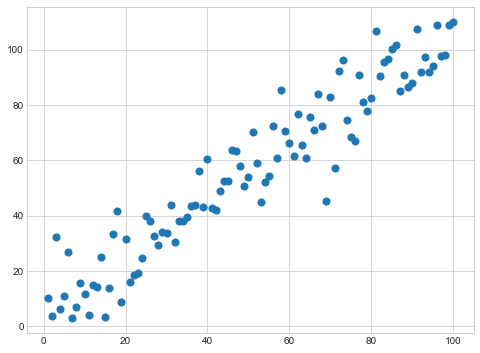
\includegraphics[scale=0.4]{regr_pic_1.png}
\end{minipage}
\hfill
\begin{minipage}[t]{0.45\textwidth}
	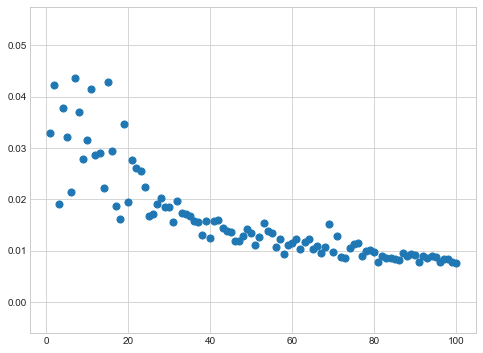
\includegraphics[scale=0.4]{regr_pic_2.png}
\end{minipage}

\begin{minipage}[t]{0.45\textwidth}
	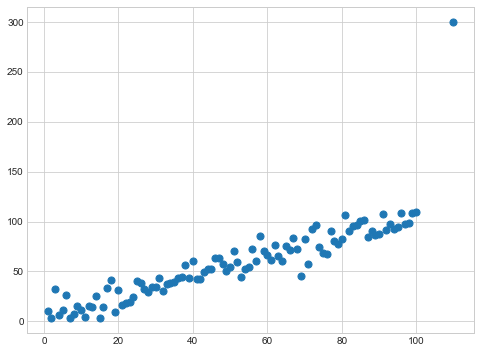
\includegraphics[scale=0.4]{regr_pic_3.png}
\end{minipage}
\hfill
\begin{minipage}[t]{0.45\textwidth}
	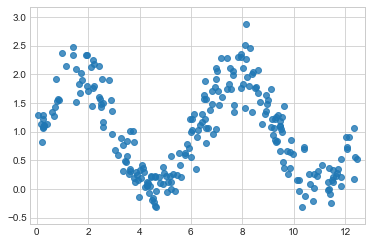
\includegraphics[scale=0.55]{regr_pic_4.png}
\end{minipage}

\begin{enumerate}	
	\item[а)] Нарисуйте на каждой из картинок линию регрессии.
	\item[б)] Как выглядят уравнения регрессии в этих ситуациях? Какие параметры в них нам нужно обучить?
	\item[в)] В чём проблема на картинке слева снизу? Проинтерпретируйте её на примере шашлыков.
	\item[г)] В четвёртой ситуации мы выбрали для обучения полином. А почему бы не взять его в каждой ситуации и не обучить через каждую точку? 
	\item[д)] Ещё одна, на этот раз трёхмерная картинка! Слабо дополнить её также, как мы делали это выше? Как будет выглядеть уравнение регрессии?
\end{enumerate}

\begin{center}
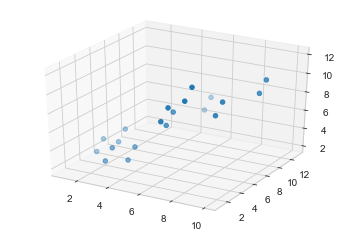
\includegraphics[scale=0.8]{regr_pic_5.png}
\end{center}


\ifbool{answers}{
	\textbf{Решение:}
	
	
\begin{enumerate}	
	\item[а)] Берём и рисуем! 
	
	\begin{minipage}[t]{0.45\textwidth}
		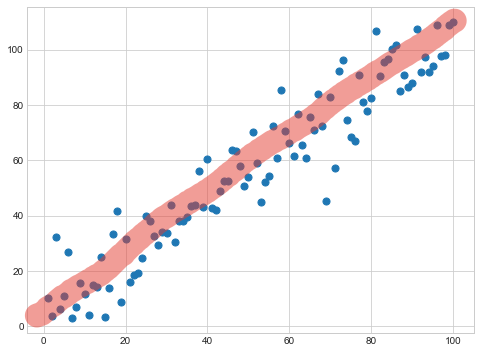
\includegraphics[scale=0.4]{regr_pic_1_ans.png}
	\end{minipage}
	\hfill
	\begin{minipage}[t]{0.45\textwidth}
		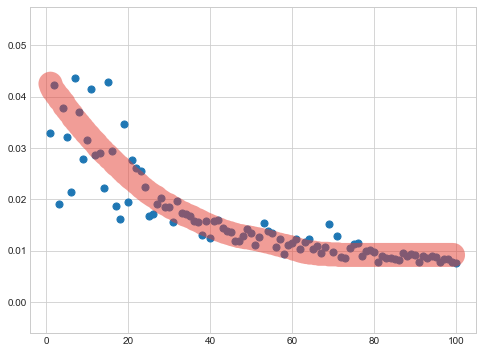
\includegraphics[scale=0.4]{regr_pic_2_ans.png}
	\end{minipage}
	
	\begin{minipage}[t]{0.45\textwidth}
		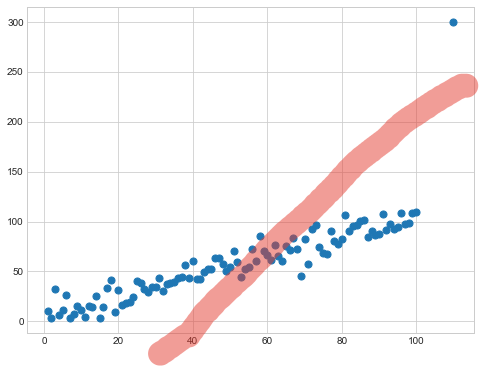
\includegraphics[scale=0.4]{regr_pic_3_ans.png}
	\end{minipage}
	\hfill
	\begin{minipage}[t]{0.45\textwidth}
		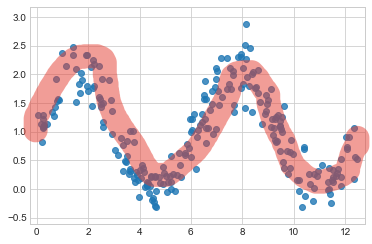
\includegraphics[scale=0.55]{regr_pic_4_ans.png}
	\end{minipage}
	
	
	\item[б)]  В первой ситуации это обычная линейная модель $y_i = \beta_0 + \beta_1 x_i$. Во второй ситуации перед  нами нелинейная модель. Внешне картинка похожа на гиперболу. Можно попробовать обучить модель $y_i = \frac{1}{\beta_0 + \beta_1 x_i}$. Однако на практике обычно поступают иначе. Если взять от $x_i$ логарифм, то модель стане линейной, и модно будет обучить $y_i = \beta_0 + \beta_1 \ln x_i$. В третьей ситуации это снова обычная линейная модель. В четвёртой ситуации это либо многочлен, либо какой-нибудь косинус. Об этих двух ситуациях мы поговорим подробнее ниже. 
	
	\item[в)]  Это толстый друг, который много ест.  Он портит обучение модели и прямая, вместо того, чтобы пройти через облако точек, подстраивается под него. Такие ситуации обычно называют выбросами. Если последовать рецепту из первого упражнения и наложить на тостого друга дамми, то ситуация нормализируется, и красная прямая пройдёт сквозь облако также как и в первой ситуации. Это эквивалентно тому, что мы выбрасываем друга из выборки и работаем с ним отдельно.
		
	Другой путь: использовать модели, которые нечувствительны к выбросам. В ходе этого семинара вы столкнётесь с двумя такими моделями.
	
	\item[г)]  В четвёртой ситуации мы взяли полином. Возможно, у вас возник соблазн обучить и в первых трёх ситуациях модель, которая пройдёт через все возможные точки. Это неправильно. В таком случае наша модель слишком сильно вылизывает данные. Обычно в них много шума, и модель подстраивается под него, вместо того, чтобы вычленить сигнал. Это обычно называют переобучением.
	
	\item[д)]  В этой ситуации мы строим модель не на одну переменную ($y$ на $x$), а на две ($y$ на $x$ и на $z$). Уравнение будет иметь вид $y_i = \beta_0 + \beta_1 \cdot x_i + \beta_2 \cdot z_i$. В алгебре такое уравнение описывает двумерную плоскость в трёхмерном пространстве. Новость: в трёхмерном случае мы учим не линию, а плоскость. Если размерность пространства ещё больше, мы учим некоторую гиперплоскость. 
	
	 \begin{center}
	 	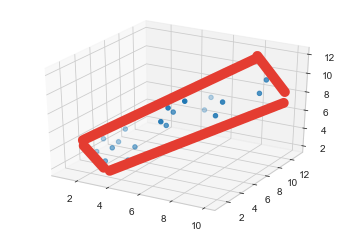
\includegraphics[scale=0.8]{regr_pic_5_ans.png}
	 \end{center}
	
\end{enumerate}
}


\subsection*{Задача 3}

Вася измерил вес трёх упаковок с конфетками,  $y_1=6$, $y_2=6$, $y_3=10$.  Вася хочет спрогнозировать вес следующего пакетика. Модель для веса пакетиков у Васи очень простая, $y_i = \mu + u_i$, поэтому прогнозирует Вася по формуле $\hat y_i = \hat \mu$.

Для оценки параметра $\mu$ Вася использует следующую целевую функцию:
\[
\sum (y_i - \hat \mu)^2 + \lambda \cdot \hat \mu^2
\]

\begin{enumerate}
	\item[a)] Найдите оптимальное $\hat\mu$ при $\lambda =0$.
	\item[б)] Найдите оптимальное $\hat\mu$ при произвольном $\lambda$.
	\item[в)] Подберите оптимальное $\lambda$ с помощью кросс-валидации «выкинь одного».
	\item[г)] Найдите оптимальное $\hat\mu$ при $\lambda_{CV}$.
\end{enumerate}

\ifbool{answers}{
	\textbf{Решение:}
	
\begin{enumerate}
	\item[a)]  В пункте а Вася хочет подобрать модель, которая будет прогнозировать вес нового пакетеки с конфетками. Для этого он руководствуется принципом минимизации квадрата ошибки. Если бы Вася спрогнозировал, что первый пакетик будет весить $\mu$, он бы ошибся на $(6 -  \mu)^2$. Если бы Вася спрогнозировал, что второй пакетик будет весить $\mu$, он бы ошибся на $(6 - \mu)^2$.  В случае третьего пакетика ошибка составила бы $(10 -  \mu)^2$.  Наша дальнейшая задача --- минимизируя суммарную ошибку Васи, получить хорошую оценку для $\mu$: 
	
	\[L(\mu) = (6 - \mu)^2 + (6 -  \mu)^2 + (10 -  \mu)^2 \to \min_{ \mu}.\]
	
	Давайте вспоминать 11 класс школы. ОХ! Как же давно это было. Как найти экстремум функции? Взять производную и приравнять её к нулю! 
	
	\[  -4 \cdot (6 - \mu) - 2 \cdot (10 - \mu) = 0 \Rightarrow \hat \mu = \frac{44}{6} \approx 7.3. \]
	
	Итак, если Вася хочет строить для каждого последущего пакетика прогнозы с помощью одного числа, и при этом он минимизирует квадратичную ошибку, наименьшие потери даст прогноз $7.3$. Если конечно верить данным. 
	
	Если нарисовать $L(\mu)$ на картинке, то можно увидеть, что минимум ошибки, действительно, достигается в точке $7.3$.
	
	\begin{center}
		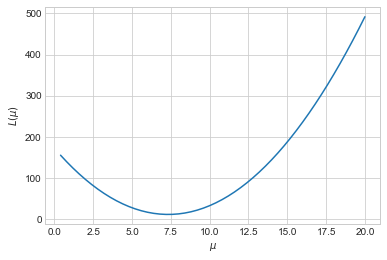
\includegraphics[scale=0.6]{mul.png}
	\end{center}
	
	
	\item[б)]  Усложняем задачу. Теперь мы обучаем модель, но уже  с гиперпараметром $\lambda$. Правда непонятно нафига нам этот гиперпараметр сдался. Давайте попробуем точно также, как в предыдущем пункте, минимизировать ошибку с участием гиперпараметра и посмотреть на то как наши прогнозы $\mu$ зависят от него. 
	
		\[L(\mu) = (6 - \mu)^2 + (6 -  \mu)^2 + (10 -  \mu)^2 + \lambda \mu^2 \to \min_{ \mu}.\]
		
	Снова берём производную. Всё, как в школе учили. 
	
\begin{equation*}
\begin{aligned}
	&-4 \cdot (6 - \mu) - 2 \cdot (10 - \mu) + 2 \mu \lambda = 0  \\
	&44 = 6 \mu + 2 \lambda \mu \\
	&22 = 3 \mu + \lambda \mu \\
	&22 = \mu(3 + \lambda) \\
	&\hat \mu = \frac{22}{3 + \lambda}
\end{aligned}
\end{equation*}
	
Отлично. Теперь у нас есть зависимость наших прогнозов от гиперпараметра в явном виде. Давайте попробуем посмотреть как выглядит эта зависимость на графике. 	

\begin{center}
	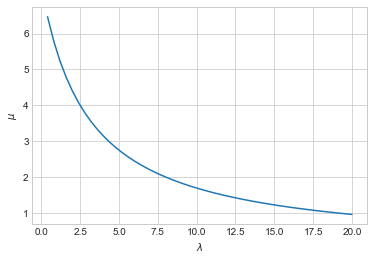
\includegraphics[scale=0.6]{lambda_mu.png}
\end{center}

Гиперпараметр лямбда обладает интересным эффектом. Он зануляет значение $\mu$, если оказывается очень большим.  Именно так работает регуляризация. Она стягивает коэффициенты к нулю. Когда модель слишком сильно подстраивается под данные, коэффициенты в ней оказываются очень большими (вспомните картинку из второго задания). Стягивание к нулю запрещает модели слишком сильно подстраиваться под данные. 

\item[в)]   Получается, что меняя гиперпараметр $\lambda$, мы можем давать бой переобучению модели и, варьируя его, улучшать прогнозную силу. Возникает вопрос: а как выбрать оптимальное значения для $\lambda$? Давайте вспомним предыдущий семинар и то, как мы делали это с муравьями, когда подбирали оптимальное число соседей для нашего алгоритма. 
	
	Мы закрывали одного муравья ладошкой, на оставшихся обучали классификатор, а затем смотрели куда будет относиться закрытый ладошкой муравей. Сделав так с каждым муравьём, мы смотрели сколько ошибок допустили при $k=3$ и при $k=4$, и брали такое $k$, для которого ошибок было меньше. Говоря иначе, мы с помощью кросс-валидации <<выкинь одного>> по решётке подобрали оптимальное значение для гиперпараметра $k$, которое позволило нам получить хорошие прогнозы.
	
	Здесь нам надо будет сделать аналогичным образом.  Нам придётся перебрать все возможные значения $\lambda$, закрывая каждое из трёх наблюдений, по очереди, ладошкой.  Сделаем это для всех возможных $\lambda$ и посмотрим на суммарную ошибку. 
	
	Закрываем ладошкой третье наблюдение. Это означает, что наша модель будет оцениваться по первым двум наблюдениям. То есть
	
	\[L(\mu) = (6 - \mu)^2 + (6 -  \mu)^2  \lambda \mu^2 \to \min_{ \mu}.\]
	
	Берём производную, решаем уравнение, получаем, что $\hat \mu = \frac{12}{2 + \lambda}$. На закрытом от наших глаз наблюдении мы хотим проверить работоспособность модели. Ошибка модели составит
	
	\[ \left( 10 - \frac{12}{2 + \lambda}  \right)^2. \] 
	
	Закрываем ладошкой второе наблюдение. Модель оценивается по первому и третьему наблюдениям. То есть
	
		\[L(\mu) = (6 - \mu)^2 + (10 -   \mu)^2  \lambda \mu^2 \to \min_{ \mu}.\]
		
	Берём производную, решаем уравнение, получаем, что $\hat \mu = \frac{16}{2 + \lambda}$. Ошибка на оставшемся наблюдении составит
	
		\[ \left( 6 - \frac{16}{2 + \lambda}  \right)^2. \] 
	
	Закрываем ладошкой первое наблюдение. Из-за того, что оно совпадает со вторым, получаем такой же результат. Получается, что суммарная ошибка для произвольного $\lambda$, посчитанная по кросс-валидации <<выкинь одного>> составит 
	
	\[ 2\cdot \left( 6 - \frac{16}{2 + \lambda}  \right)^2  +  \left(10 -  \frac{12}{2 + \lambda}  \right)^2. \]	

	Если подставлять в эту формулу разные $\lambda$, мы будем получать разные ошибки. Нам хочется подобрать оптимальное $\lambda$, при котором ошибка будет наименьшей. Как это сделать? Ещё разок взять производную! 
	
	Для удобства сделаем замену $t = \frac{4}{2 + \lambda}$ и будем минимизировать функцию 
	
		\[ 2(6 - 4t)^2 + (10 - 3t)^2 \to \min_t. \]	
		
	Возьмём производную, приравняем к нулу, получим, что $t = \frac{78}{41}$. Дело осталось за малым, восстановить $\lambda$:
	
\begin{equation*}
\begin{aligned}
&t = \frac{4}{2 + \lambda}, \\ 
&\frac{78}{41}  = \frac{4}{2 + \lambda}, \\
&39 \cdot(2 + \lambda) = 82,\\ 
&\lambda = \frac{82 - 78}{39} = \frac{4}{39}.\\
\end{aligned}
\end{equation*}	

Получается, что гиперпараметр $\lambda^{cv} = \frac{4}{39}$ будет минимизировать ошибку на валидации, и именно его имеет смысл использовать при построении прогнозов. 

\item[г)] Наконец-то пришло время выяснить каким будет вес следущей пачки конфеток. 

\[ \hat \mu = \frac{22}{3 + \frac{4}{39}} = 7.09.\]
	
После того, как мы ввели в модель гиперпараметр $\lambda$ и подобрали его с помощью кросс-валидации, он стянул оптимальное значение $\mu$ чуть ближе к нулю. Это произошло из-за того, что $10$ в данной выборке является в какой-то степени аномальным весом конфеток. Она перетягивает на себя величину прогноза и модель переобучается под десятку. Введение лямбды позволяет немного вылечить это переобучение и вернуть прогнозы ближе к $6$. Модель с регуляризатором считает, что отклонение в сторону $10$ это аномалия, и обращение лишнего внимания на неё испортит дальнейшие прогнозы. 

Примерно так работают линейные модели машинного обучения. Разница лишь в том, что компьютер не берёт производные, а использует метод градиентного спуска.
\end{enumerate}
}


\subsection*{Задача 4}

Миша работает в маленькой кофейне. Харио Малабар Монсун является фирменным напитком этой кофейни. Мише интересно узнать как именно ведёт себя спрос на напиток $y_i$ в зависимости от температуры за окном $t_i$. Четыре дня Миша записывал свои наблюдения: 

\begin{center}
	\begin{tabular}{c|c}
		\hline
		$t_i$ & $y_i$ \\
		\hline
		21 &  1 \\
		19 & 2 \\
		12 & 8 \\
	     8 & 8 \\
	\end{tabular}
\end{center}

Сегодня он решил обучить регрессионное дерево. В качестве функции потерь он использует 

\[ \sum (y_i - \hat y_i)^2. \]

\begin{enumerate}
	\item[а)] Обучите регрессионное дерево.
	\item[б)] Какой прогноз на сегодня сделает дерево Миши, если за окном $13$ градусов? 
\end{enumerate}


\ifbool{answers}{
	\textbf{Решение:}
	
На этом семинаре мы сажаем дерево. Будем ли мы на следущем строить дом и рожать ребёнка --- большой вопрос.  Мы должны по переменной $t$ спрогнозировать переменную $y$. Для этого нужно обучить дерево. Учить мы его будем по-жадному. Будем смотреть какое разбиение по переменной $t$ сильнее всего уменьшает ошибку, и выбирать его. 

На первом шаге у нас есть три способа сделать разбиение по переменной $t$: 
\begin{center}
	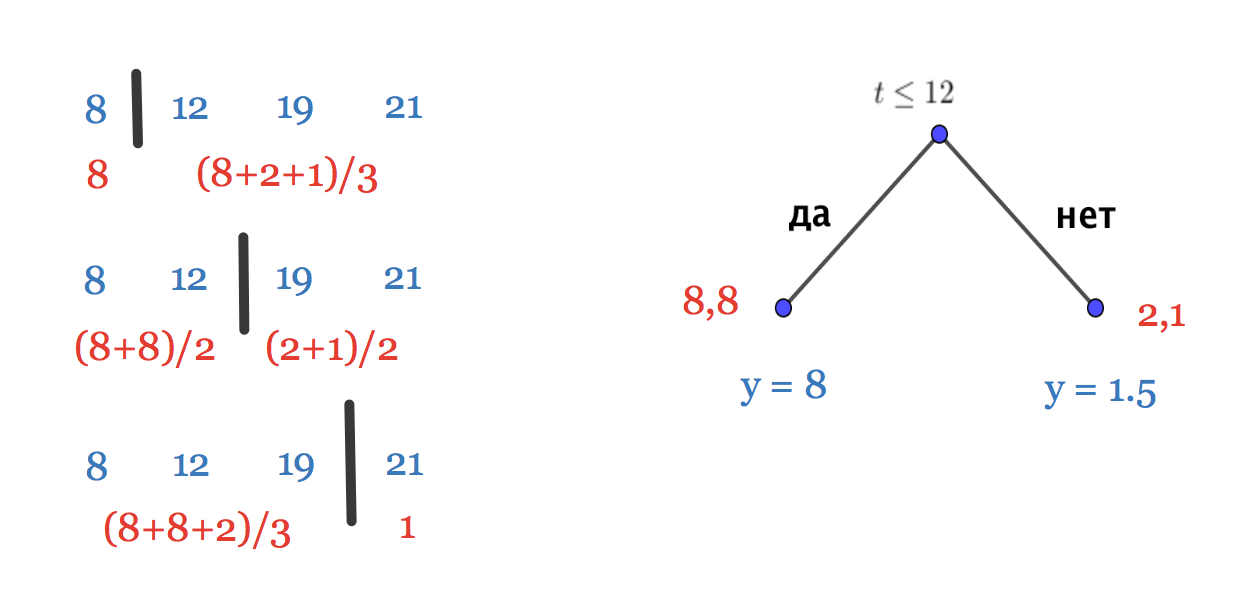
\includegraphics[scale=0.25]{reg_tree_1.png}
\end{center}

	\begin{itemize}
		\item  	Мы можем отправть  в левую вершину все ситуации, где температура меньше либо равна 8 градусам. В таком случае, когда мы идём по дереву налево, мы будем прогнозировать, что потребители выпьют $8$ чашек кофе. Когда мы идём вправую вершину, мы будем прогнозировать, что потребители выпьют $3.6$ чашек кофе. Это среднее всех $y$, попавших в правую вершину. Давайте посчитаем ошибку, которую при этом будет допускать дерево. 
		
		\[ (8 - 8)^2 + (8 - 3.6)^2 + (2 - 3.6)^2 + (1 - 3.6)^2 = 28.68.  \]
		
		\item Мы можем отправить в левую вершину все ситуации, где температур меньше либо равна $12$. В таком случае слева прогноз будет $8$, а справа $1.5$. Найдём ошибку:
		
		\[ (8 - 8)^2 + (8 - 8)^2 + (2 - 1.5)^2 + (1 - 1.5)^2 = 0.5.  \]
		
		\item В третьей ситуации получаем, что 
		
		\[ (8 - 6)^2 + (8 - 6)^2 + (2 - 6)^2 + (1 - 1)^2 = 24.  \]
	\end{itemize}

Оптимальным для разбиения оказывается второй вариант. Он сильнее всего уменьшает ошибку.  Выбрав его, мы отправляем влевую вершину две восьмёрки и получаем в ней нулевую ошибку. Вправую вершину мы отправляем двойку и единицу. 

В правой вершине нужно сделать ещё одну итерацию, чтобы отделить двойку от единицы. Тогда обучение дерева будет окончено. Итоговое дерево будет иметь вид: 

\begin{center}
	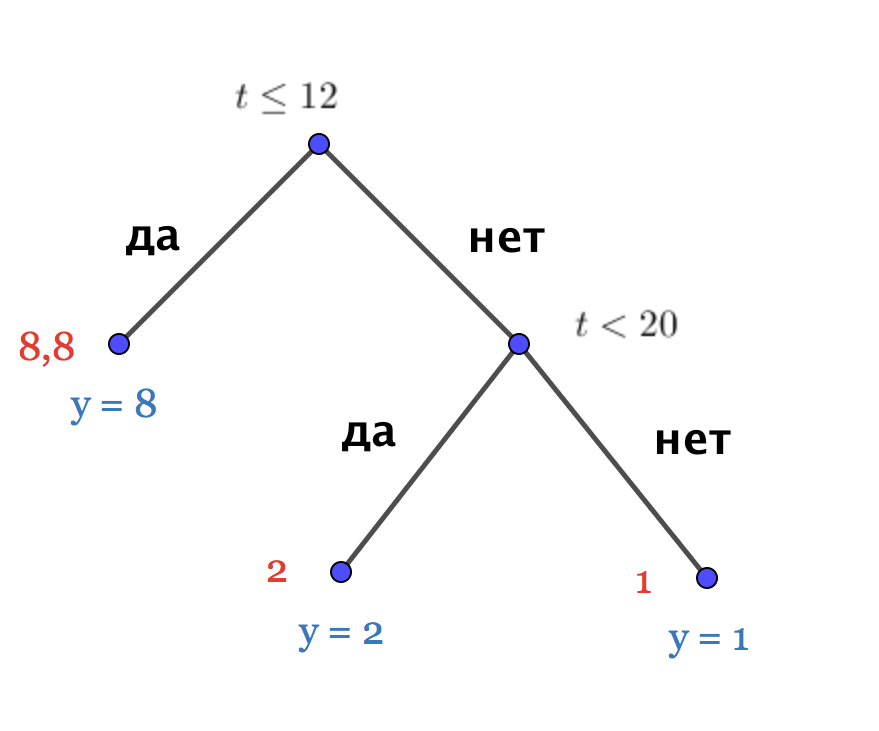
\includegraphics[scale=0.23]{reg_tree_2.png}
\end{center}

Сделаем прогноз для $13$ градусов.  Для этого пройдёмся по дереву от корня к одному из листов. На улице меньше или равно $12$ градусов?  нет. Идём направо. На улице меньше $20$ градусов? Да. Идём налево. В кофейне купят $2$ чашки. 

Обратите внимание, что дерево идеально запомнило обучающую выборку. Оно слишком сильно фрагментировало её. Это является переобучением. Чтобы деревья не переобучались и не вылизывали выборку, обычно останавливают обучение деревьев досрочно: 

\begin{itemize} 
	\item  Когда в вершини оказалось не менее $10$ объектов
	\item  Когда дерево построилось до $20$ листьев. 	
	\item  Когда глубина дерева оказалась равна $5$.
\end{itemize}

Конечно же конкретные цифры здесь для пример. Они являются гиперпараметрами и подбираются также как мы подбирали $k$ в методе ближайших соседей на предыдущем семинаре. Другой путь --- применять сразу много деревьев. Примером такой модели является случайный лес.  
}


\subsection*{Задача 5}

Предположим, что в наших руках оказались исторические данные по продажам $45$ магазинов Walmart, расположенных в разных регионах. Каждый магазан содержит несколько отделов.  Нам хотелось бы научиться прогнозировать продажи по каждому отделу. 

\begin{enumerate}
	\item[а)]  Зачем нам может понадобиться прогнозировать продажи? Какая от этого выгода для магазина? 
	\item[б)] Какую задачу машинного обучения нам предстоит решать? Какие переменные мы могли бы использовать в качестве объясняющих? 
	\item[в)] Какую метрику мы могли бы использовать для оценки бизнес-эффекта от нашей модели? Отталкиваясь от каких характеристик можно было бы сконструировать её? 
	\item[г)]  Что такое MAE, MSE,  RMSE и MAPE?  Предположим, что у нас есть три магазина. Они продали товаров на $5$, $10$ и $100$  рублей.  Наша модель предсказывала, что они продадут товаров на  $4$, $20$ и $110$. Посчитайте для нашей модели все четыре метрики качества, приведённые выше. 
\end{enumerate}


\ifbool{answers}{
	\textbf{Решение:}

Все пункты мы подробно обсудили на семинаре. Это задача является вводной к юпитерской тетрадке. В ней всё подробно расписано. Та же подробно можно прочесть про метрики. Здесь будет только решение только пункта г). 

\begin{equation*}
\begin{aligned}
&MAE = \frac{1}{3} \cdot( |5 - 4| + |10 - 20| + |100 - 110| )= 7 \\
&MSE = \frac{1}{3} \cdot(  (5-4)^2 + (10 - 20)^2 + (100 - 110)^2) = 67 \\
&RMSE = \sqrt{MSE} \approx 8.19 \\
&MAPE = 100\cdot \frac{1}{3} \cdot\left( \frac{|5 - 4|}{5} + \frac{|10 -20|}{10} + \frac{|100 - 110|}{100} \right) =  43 \% \\
\end{aligned}
\end{equation*}	
}


\section*{Ещё задачи}

\subsection*{Задача 6}

Маркетологи Вова и Вася строили регрессию $y = \beta_0 + \beta_1 x$. Каждый оценивал её по своим данным. У Васи получилось, что $\hat \beta_1 = 2$, у Вовы получилось, что $\hat \beta_1 = 8$.

Пришла Алиса, отобрала у Вовы и Васи данные, соединила их вместе и построила регрессию сразу на всём. У неё получилось, что $\hat \beta_1 = -10$. Может ли такое быть?


\ifbool{answers}{
	\textbf{Решение:}
	
Конечно может быть! Надо лишь немного пофантазировать.  Пусть выборки Васи и Вовы имеют следущий вид: 

\begin{center}
	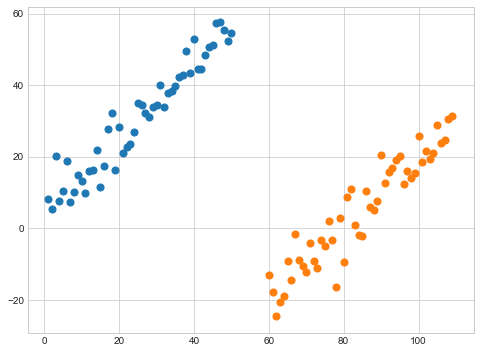
\includegraphics[scale=0.5]{VVA_1.png}
\end{center}

Если они попробуют построить свои линии регрессии, они получат положительные коэффициенты наклона. При этом, если неожиданно придёт Алиса и отберёт у них выборки, она получит отрицательный наклон у своей прямой.

\begin{center}
	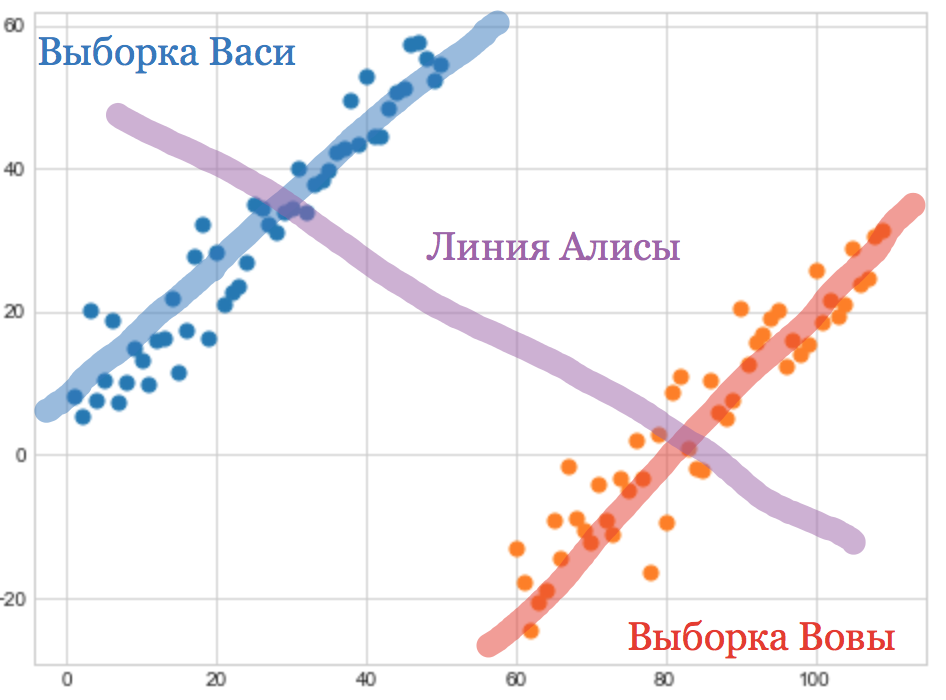
\includegraphics[scale=0.25]{VVA_2.png}
\end{center}
	
}


\subsection*{Задача 7}

Выращиваем регрессионное дерево в домашних условиях! Вот вам выборка для этого: 

\begin{center}
	\begin{tabular}{c|c}
		\hline
		$x_i$ & $y_i$ \\
		\hline
		0 & 5 \\
		1 &  6\\
		2 & 4 \\
		3 & 100 \\
	\end{tabular}
\end{center}

Критерий деления вершины --- минимизация квадратичной функции потерь. Критерий остановки --- три листа.  Зачем нужен критерий остановки? Как дерево ведёт себя с выбросами? 

\ifbool{answers}{
	\textbf{Решение:}
	
У нас есть три способа раздробить по $x$ дерево. 

\begin{center}
	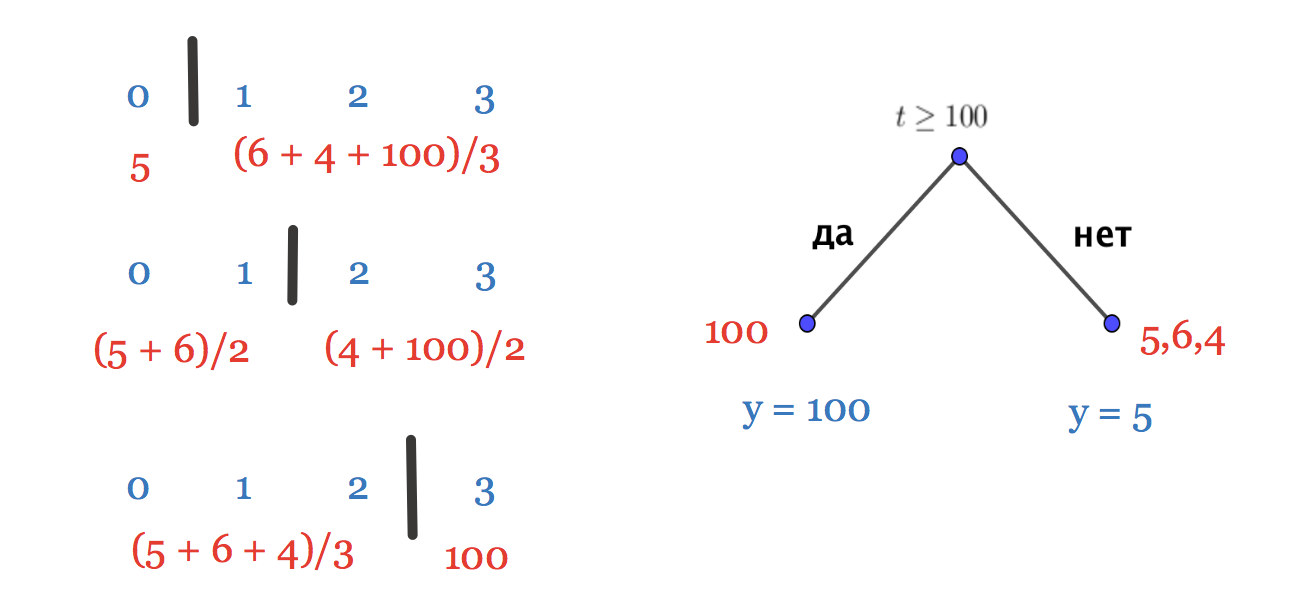
\includegraphics[scale=0.25]{reg_tree_3.png}
\end{center}

Посчитаем для каждого способа квадратичную ошибку: 

\begin{itemize}
	\item  $ (5 - 5)^2 + (6 - 36.6)^2 + (4 - 36.6)^2 + (100 - 36.6)^2 = 6018.68$
	\item  $ (5 - 5.5)^2 + (6 - 5.5)^2 + (4 - 52)^2 + (100 - 52)^2 = 4608.5$
	\item  $ (5 - 5)^2 + (6 - 5)^2 + (4 - 5)^2 + (100 - 100)^2 = 2$
\end{itemize}

Выгоднее всего оказывается обособить первым же отсечением выброс. Это нормальная ситуация. На практике так происходит регулярно. Деревья изолируют выбросы в отдельные вершины, и они никак не портят работу с основной выборкой. Такое свойство называется нечувствительностью к выбросам или робастностью к выбросам. В следущем упражнении, мы с вами встретимся с ещё одной моделью, которая устойчива к выбросам. 

Сделаем второй шаг разбиения. 

\begin{center}
	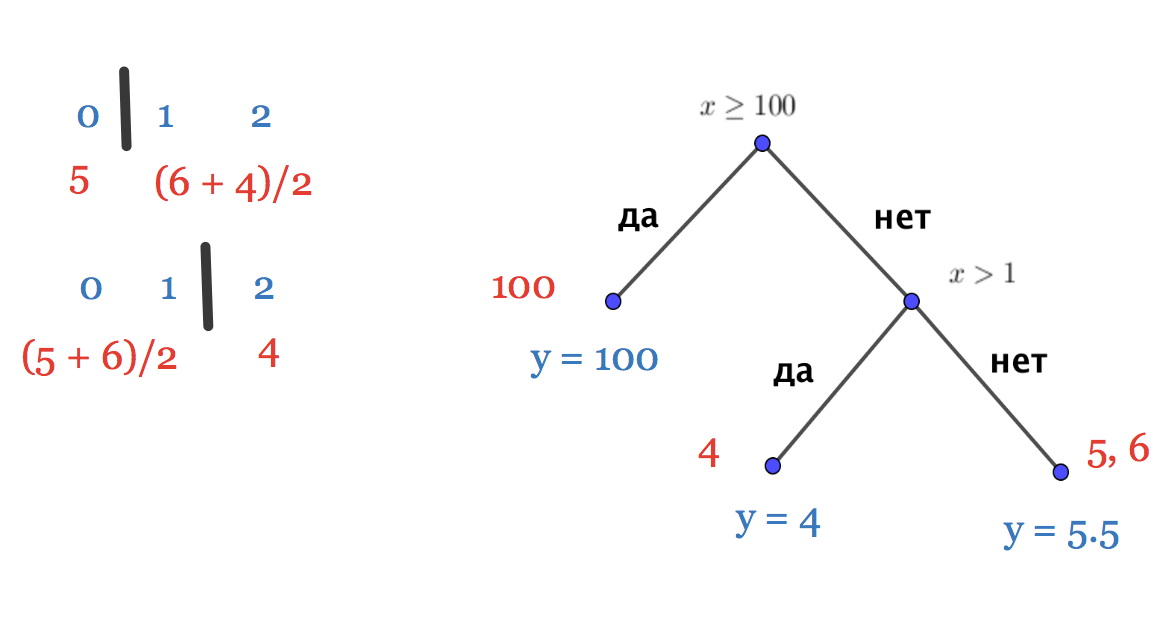
\includegraphics[scale=0.25]{reg_tree_4.png}
\end{center}

Посчитаем для каждого способа квадратичную ошибку: 

\begin{itemize}
	\item  $ (5 - 5)^2 + (6 - 5)^2 + (4 - 5)^2 = 2$
	\item  $ (5 - 5.5)^2 + (6 - 5.5)^2 + (4 - 4)^2  = 0.5$
\end{itemize}
	
Понятно, что дробить нужно, обосабливая четвёрку. После этого нужно остановиться. По условию задачи критерий остановки --- три листа у дерева. Ошибка бы продолжила убывать для тренировочной выборки. На тестовой она бы возрастала. Обычно подобные критерии ранней остановки помогают избежать переобучения.
	
Кстати говоря, именно благодаря тому, что деревья на первом же шаге изолируют выбросы, случайный лес можно из прогнозной модели модернизировать в модель, которая неплохо справляется с поиском аномалий. Подумайте на досуге как именно можно сделать это. 
}



\subsection*{Задача 8}

Каждый день Маша ест конфеты и решает задачи по машинному обучению. Пусть $x_i$ — количество решённых задач, а $y_i$ — количество съеденных конфет.

\begin{center}
\begin{tabular}{c|c}
	\hline
	$x_i$ & $y_i$ \\
	\hline
	1 & 1 \\
	2 & 2 \\
	2 & 8 \\
\end{tabular}
\end{center}

Рассмотрим модель $y_i = \beta x_i + u_i$. Маша использует функцию потерь 
\[
\sum (y_i - \hat \beta x_i )^2
\]

\begin{enumerate}
	\item[а)] Найдите МНК-оценку $\hat \beta$ для имеющихся трёх наблюдений.
	\item[б)] Нарисуйте исходные точки и полученную прямую
	регрессии.
	\item[в)] Выведите формулу для $\hat \beta$ в общем виде для $n$ наблюдений.
	\item[г)] На семинаре по машинному обучению неожиданно выяснилось, что Миша тоже каждый день решает задачи по машинному обучению. Правда он более сдержан в плане конфет. Миша решил взять Машины наблюдения и с помощью функционала 
	\[
	\sum |y_i - \hat \beta x_i |
	\]  
	
	оценить $\beta$. Помогите Мише найти оценку. 
	\item[д)] К поеданию конфет решает присоединиться Вадик. У него тоже есть своя функция потерь
	\[
	\sum (y_i - \hat \beta x_i)^2 + 3\beta^2
	\]  	
	Оцените $\beta$ для его случая. Нарисуйте все три прямые на одной картинке и порассуждайте почему они получились именно такими, какими получились. 
\end{enumerate}

\ifbool{answers}{
	\textbf{Решение:}
	
\begin{enumerate}
	\item[а)] Текущая модель немного посложнее модели из третьей задачи. Тем не менее, она решается ровно по такой же схеме. Выписываем ошибку и минимизируем её по параметрам модели: 
	
	\[ (1- \beta)^2 + (2 - 2 \beta)^2 + (8 - 2 \beta)^2 \to \min_{\beta} \]
	
	Берём производную и приравниваем её к нулю: 
		
	\begin{equation*}
	\begin{aligned}
	& -2(1-\beta) - 4(2-2\beta) - 4(8-2\beta) = 0, \\
	& (1-\beta) + 2(2 - 2 \beta) + 2(8 - 2 \beta) = 0, \\
	&  9 \beta = 21, \\
	&  \hat \beta = \frac{21}{9}.\\
	\end{aligned}
	\end{equation*}	
	
	Итоговая модель для строительства прогнозов: $y = \frac{21}{9} \cdot x$. Обратите внимание, что в данном случае мы оценивали именно зависимость $y$ от $x$. Для каждого $x$ будет свой прогноз $y$. 
	
	\item[б)]  Написуем наши наблюдения и оценённую прямую на одной картиночке! 
	
	\begin{center}
		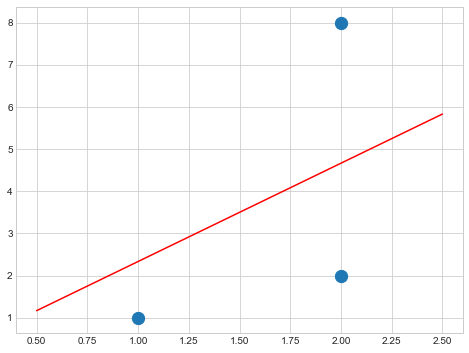
\includegraphics[scale=0.5]{reg_81.png}
	\end{center}
	
	
	\item[в)]  Выведем формулу для случая $n$ наблюдений. Ошибка будет иметь вид: 
	
	\[(y_1 - \beta x_1)^2 + (y_2 - \beta x_2)^2 + \ldots + (y_n - \beta x_n )^2 \to \min_{\beta} \]
	
	Берём производную! 
	
	\begin{equation*}
	\begin{aligned}
	&  -2 x_1 (y_1 - \beta x_1) - 2 x_2 (y_2 - \beta x_2) - \ldots -2 x_n (y_n - \beta x_n) = 0 \\
	& x_1 (y_1 - \beta x_1) +  x_2 (y_2 - \beta x_2) + \ldots +  x_n (y_n - \beta x_n) = 0  \\
	& x_1 y_1 - \beta x_1^2 + x_2 y_2 - \beta x_2^2 + \ldots + x_n y_n - \beta x_n^2 = 0\\
	& x_1 y_1 + \ldots + x_n y_n = \beta (x_1^2 + \ldots + x_n^2) \\
	\end{aligned}
	\end{equation*}
	
	В итоге получаем, что $\hat \beta = \frac{x_1 y_1 + \ldots + x_n y_n}{x_1^2 + \ldots + x_n^2}$ или, более лаконично записывая, $\hat \beta = \frac{\sum_{i=1}^{n} x_i y_i }{\sum_{i=1}^n x_i^2}.$
	
	\item[г)] Выписываем ошибку Миши
	
	\[ |1- \beta| + |2 - 2 \beta| + |8 - 2 \beta|  \to \min_{\beta}. \]
	
	У нас проблемы. От модуля нельзя взять производную. К счастью, у нас мало наблюдений и и мы можем нарисовать нашу функцию потерь. Она будет кусочно-линейной. У неё будет две особые точки: $1$ и $8$.  Посмотрим как ведёт себя наша функция до точки $1$. Раскрываем модули и получаем поведение функции на промежутке от минус бесконечности до $1$: 
	
	\[ 1 - \beta + 2 - 2\beta + 8 - 2\beta = 11 - 5\beta.\] 	
	
	Теперь раскрываем модули на отрезке от $1$ до $8$: 
	
	\[ - 1 + \beta - 2 + 2\beta + 8 - 2\beta = 5 + \beta.\] 
	
	Раскрываем модули на промежутке от $8$ до конца: 
	
	\[ - 1 + \beta - 2 + 2\beta  - 8 + 2\beta = -11 + 5 \beta. \]
	
	Изобразим нашу функцию потерь на картинке. 
	
	\begin{center}
		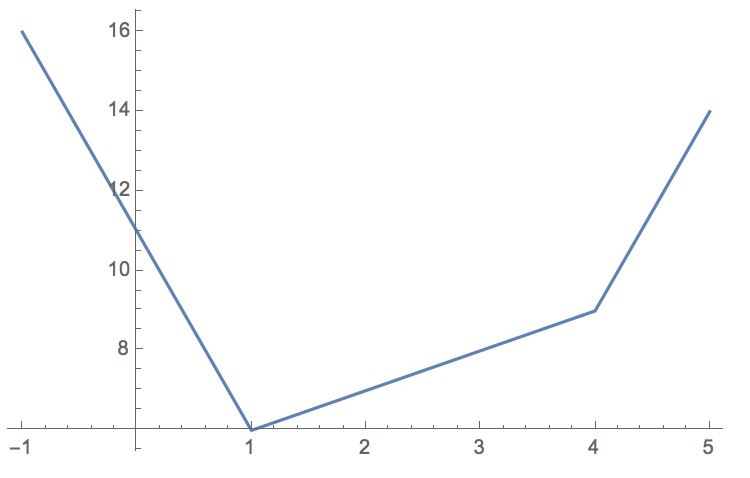
\includegraphics[scale=0.4]{reg_82.png}
	\end{center}
	
	Функция достигает минимума в точке $1$, получается что $\hat \beta = 1$. 
	
	\item[д)]  У Вадика модель с регуляризатором. Не факт, что $\lambda$ в его случае выбрана оптимально. При желании можно попробовать подобрать оптимальное значение, используя ту же стратегию, что и в третьей задаче. Минимизируем ошибку Вадика. 
	
		\[ (1- \beta)^2 + (2 - 2 \beta)^2 + (8 - 2 \beta)^2 + 3 \beta^2 \to \min_{\beta} \]
		
	Берём производную: 
	
		\begin{equation*}
	\begin{aligned}
	& -2(1-\beta) - 4(2-2\beta) - 4(8-2\beta) + 6 \beta = 0, \\
	& (1-\beta) + 2(2 - 2 \beta) + 2(8 - 2 \beta) - 3\beta = 0, \\
	&  12 \beta = 21, \\
	&  \hat \beta = \frac{21}{12}.\\
	\end{aligned}
	\end{equation*}	
	
	Видим, что из-за наличия регуляризатора, коэффициент $\beta$ уменьшился.  Нарисуем все три линии регрессии на одной картинке и немного порассуждаем о них. 
	
	\begin{center}
		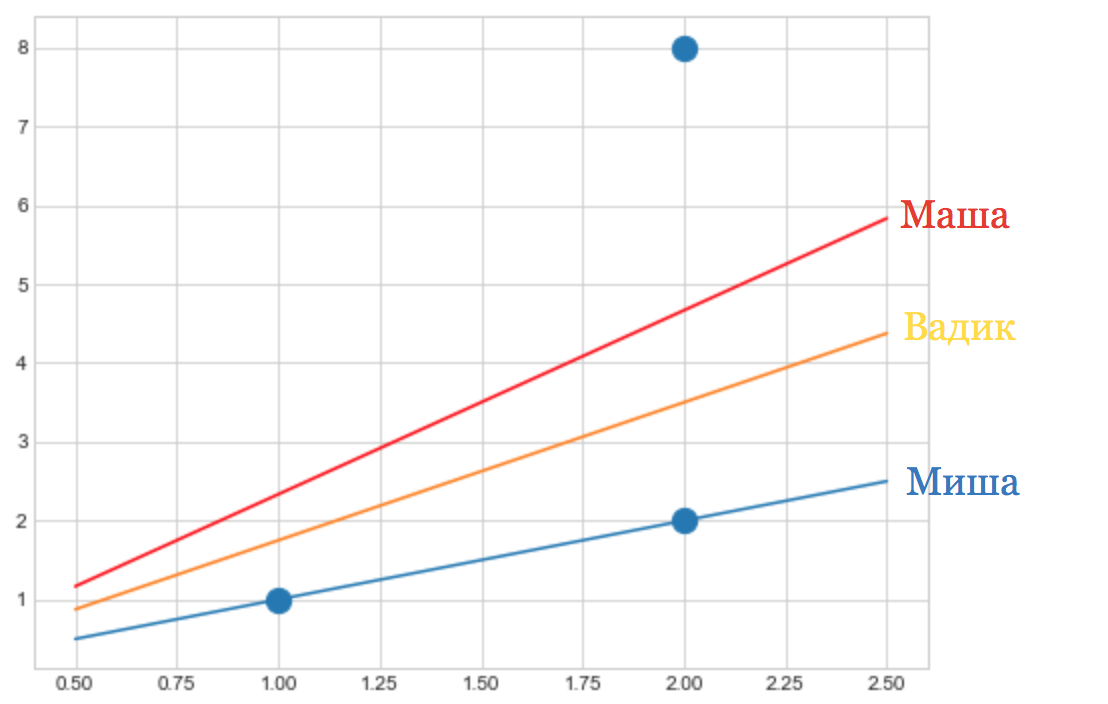
\includegraphics[scale=0.3]{reg_83.png}
	\end{center}
	
	Точка $(2,8)$ сильно выделяется. Это выброс. Машина линия довольно сильно под этот выброс подстраивается. Модель переобучается под выборку. Модель Вадика более устойчива. Из-за регуляризатора она оказывается ниже Машиной.
	
	Модель Миши оказывается удивительной. Она вообще никак не реагирует на наличие в данных выброса. Это происходит из-за того, что Миша минимизирует MAE, а остальные ребята MSE. MSE в качестве прогноза выдаёт математическое ожидание. Оно чувствительно к выбросам. MAE в качестве прогноза выдаёт медиану. Она нечувствительна к выбросам. Если вы строили модель и подозреваете, что её очень сильно портят выбросы, попробуйте использовать в качестве функции ошибки MAE вместо MSE для её обучения. 
\end{enumerate}	
}


\end{document}
